\chapter{Топология вещественной прямой}


\section*{Вводные замечания и мотивировка}

Мы начнём с рассмотрения подмножеств на числовой прямой $\mathbb{R}^1$. Напомним, что пределом последовательности $(a_n)$ называется число $a \in \mathbb{R}$, для которого верно следующее: для любого $\varepsilon >0$ найдётся такое $N$, что все $a_{N+1}, a_{N+2}, \ldots,$ принадлежат интервалу $(a -\varepsilon, a+\varepsilon).$

\begin{definition}
    Пусть $A \subseteq \mathbb{R}$. Точка $x \in \mathbb{R}$ называется \textit{предельной точкой} для множества $A$, если для любого $\varepsilon >0$, $A\setminus \{x\} \cap (x-\varepsilon, x+\varepsilon) \ne \varnothing.$ Если $A \cap (x-\varepsilon, x+\varepsilon) \ne \varnothing$, то точка $x$ называется \textit{точкой прикосновения} множества $A.$
\end{definition}

\begin{remark}
    Идея такого различия заключена в том, что нас не интересуют пределы ``почти постоянных'' последовательностей, \textit{т.е.} когда лишь конечное число её элементов различно, так что мы просим, чтобы в каждом интервале $(x-\varepsilon, x +\varepsilon)$ было ещё что-то из $A$ кроме самой точки $x.$
\end{remark}

\begin{definition}
    Пусть $A \subseteq \mathbb{R}$ -- подмножество числовой прямой. Совокупность пределов всевозможных последовательностей элементов из $A$ называется \textit{замыканием} множества $A$ и обозначается $\overline{A}.$
\end{definition}

 Таким образом, $\overline{A}$ -- это множество всех точек прикосновения множества $A$ и само множество $A$.

\begin{example}
    Пусть $A = (0,1]$, тогда ясно, что $\overline{A} = [0,1]$. Действительно, последовательность $\{\frac{1}{n}\}$ очевидно является последовательностью элементов из $A$, при этом $\lim_{n \to \infty} \frac{1}{n} = 0$. Нетрудно показать, что любой другой элемент $\alpha \in A$ также лежит в $\overline{A}$. Для этого можно рассмотреть последовательность $\{\alpha - \frac{1}{n}\}$. Таким образом, мы видим, что $A \subseteq \overline{A}$.
\end{example}

Итак, мы видим, что если задано какое-либо множество $A$ действительных чисел, то о каждом действительном числе $x\in \mathbb{R}$ можно сказать, что оно либо является предельным для $A$, либо нет. К тому же мы можем найти его замыкание используя его предельные точки. 

Рассмотрим теперь обратную задачу, \textit{т.е.} давайте в терминах замыкания сформулируем понятие предельной точки.

Итак, допустим, что для любого множества $A \subseteq \mathbb{R}$ мы знаем его замыкание $\overline{A}$. Если точка $x$ не принадлежит множеству $A$, то она будет предельной для этого множества, если и только если $x \in \overline{A}$ (ведь $\overline{A}$ и есть по определению множество всех предельных точек множества $A$).

Однако в случае, когда $x \in A$, этого критерия ($x\in \overline{A}$) уже недостаточно. Например, если $A = (0,1]\cup \{2\}$, то легко видеть, что $\overline{A} = [0,1]\cup \{2\}$. Но точка $2$ не является предельной, ведь уже интервал $(1.9, 2.1)$ не пересекается c $(0,1] = A\setminus \{2\}$.

Но, если $x \in A$ и $x$ -- предельная для $A$, то она предельная и для $A \setminus \{x\}$, то есть $x \in \overline{A \setminus \{x\}}.$

Итак, окончательно, 
\[
 \boxed{
  \boxed{ 
    \mbox{$x$ есть предельная точка для $A$} \Longleftrightarrow x \in \overline{A \setminus\{x\}}.
    } 
 }
\]

Аксиоматизируя понятие замыкания, мы приходим к понятию \textit{топологического пространства.}

\begin{definition}
   Множество $X$ называется \textit{топологическим пространством}, если каждому его подмножеству $A \subseteq X$ поставлено в соответствие множество $\overline{A}$, называемое \textit{замыканием} множества $X$, так что выполнены следующие условия:
   \begin{enumerate}
       \item $\overline{ \varnothing} = \varnothing$,
       \item $A \subseteq \overline{A}$,
       \item $\overline{A \cup B} = \overline{A} \cup \overline{B}$,
       \item $\overline{\overline{A}} = \overline{A}$.
   \end{enumerate}
\end{definition}

\begin{example}~
    \begin{enumerate}
        \item Рассмотрим $\mathbb{R}$ и рассмотрим в нём всевозможные последовательности $\{x_n\}$. Пусть $A \subseteq \mathbb{R}$, мы определим $\overline{A}$ как множество всех предельных его точек и само множество $A$.
        \item Пусть $X$ -- некоторое бесконечное множество. Определим в $X$ операцию замыкания следующими условиям: если $A$ есть конечное подмножество в $X$, то положим $\overline{A} = A$; если $A$ есть бесконечное подмножество в $X$, то положим $\overline{A} = X$. 
        \item Пусть $X$ -- некоторое множество; определим в нём операцию замыкания, положим $\overline{A} = A$ для каждого подмножества. Такое топологическое пространство называется \textit{дискретным.}
        \item Пусть $X$ -- некоторое множество; определим операцию замыкания следующим образом
        \[
         \overline{A} := \begin{cases}
             \varnothing, & A = \varnothing,\\
             X, & A \ne \varnothing.
         \end{cases}
        \]
        Такое топологическое пространство называется \textit{антидискретным.}
    \end{enumerate}
\end{example}


\section{Лекция \#10. Открытость и замкнутость}

\subsection{Открытые множества и окрестности}

\begin{definition}
    \textit{Окрестностью} точки $a \in \mathbb{R}$ радиуса $\varepsilon>0$ (=$\varepsilon$-окрестностью) называется множество
    \[
     \mathscr{B}_\varepsilon(a):=\{x\in \mathbb{R}\, :\, |x-a| < \varepsilon\} = (a-\varepsilon, a+\varepsilon).
    \]
\end{definition}

\begin{mydanger}{\bf !}
 С одной стороны, любая $\varepsilon$-окрестность любой точки -- это непустое множество, так как сама точка там находится, а с другой стороны, так как $\varepsilon>0$, то не может быть такого, чтобы $\varepsilon$-окрестность состояла всего из одной точки.
\end{mydanger}


Теперь мы введём следующее, очень важное для дальнейшего, определение.

\begin{definition}\label{open_in_R}
\textit{Открытым множеством} в $\mathbb{R}$ называется подмножество $\mathscr{U} \subseteq \mathbb{R}$, обладающее следующим свойством: для любой точки $a \in \mathscr{U}$ существует такое $\varepsilon >0$, что $\mathscr{B}_\varepsilon(a) \subseteq \mathscr{U}$.
\end{definition}

\begin{lemma}\label{point_is_not_open}
    Множество $\{a\}$ состоящее из одной точки не является открытым в $\mathbb{R}$. 
\end{lemma}

\begin{proof}
   Если бы множество $\{a\}$ было бы открыто, то для любого $x\in \{a\}$ можно было найти такую $\varepsilon$-окрестность $\mathscr{B}_\varepsilon(x)=(x-\varepsilon, x+\varepsilon)$, что $\mathscr{B}_\varepsilon(x) \subseteq \{a\}$, но множество $\{a\}$ состоит всего из одной точки, а любая $\varepsilon$-окрестность точки $a$ состоит более чем из одной точки. Поэтому включение $\mathscr{B}_\varepsilon(a) \subseteq \{a\}$ невозможно, поэтому множество $\{a\}$ не открыто.
\end{proof}

\begin{lemma}\label{interval_is_open}
Любой интервал $(a,b) \subseteq \mathbb{R}$ является открытым множеством, а тогда и всякая открытая окрестность -- это открытое множество.
\end{lemma}
\begin{proof} 
Пусть $(a,b)$ -- интервал конечной длины, тогда на него можно посмотреть как на окрестность точки $c = \frac{a+b}{2}$ (= середина отрезка) с радиусом $r = \frac{b-a}{2}$, итак
\[
 (a,b) = \mathscr{B}_r(c), \qquad c : = \frac{a+b}{2}, \qquad r: = \frac{b-a}{2}.
\]

Рассмотрим произвольную точку $x \in \mathscr{B}_r(c)$, отличную от точки $c$, \textit{т.е.} $x \ne c$ и рассмотрим её окрестность $\mathscr{B}_\delta(x)$, где $0 < \delta < r-|c-x|$. Покажем, что $\mathscr{B}_\delta(x) \subseteq (a,b)$, это и докажет требуемое.

Возьмём произвольную точку $y\in \mathscr{B}_\delta(x)$, тогда $|x-y|<\delta$, а в силу выбора $\delta$, мы также получаем, что $|x-y| < \delta < r-|c-x|.$

\begin{figure}[h!]
    \centering
    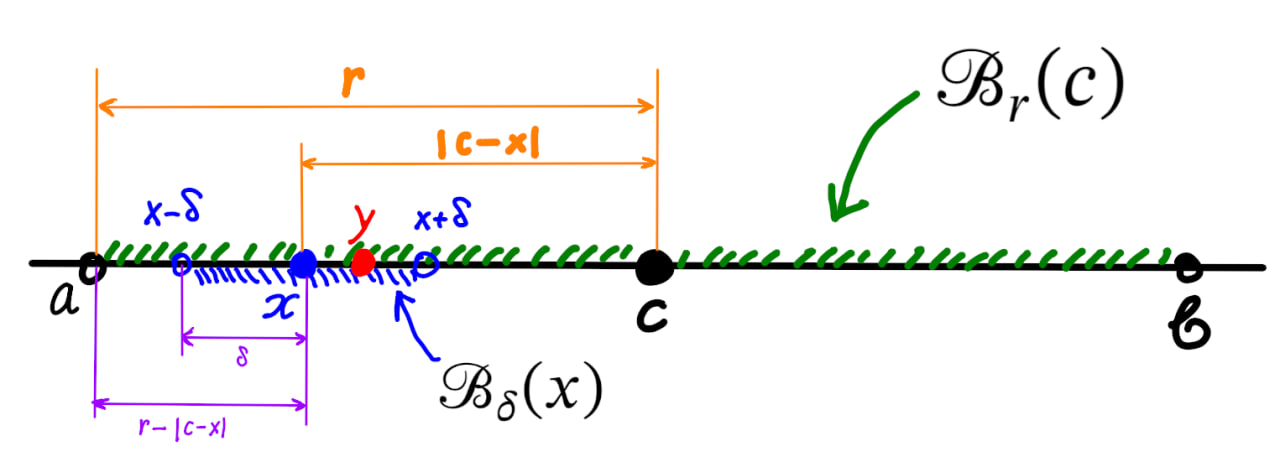
\includegraphics[scale=0.5]{images/open_is_open.jpg}
    \caption{На зелёном интервале с центром в точке $c$ мы рассматриваем произвольную синюю точку $x$ и окружаем её синей окрестностью так, чтобы она целиком была в зелёном интервале.}
    \label{fig:enter-label}
\end{figure}

Далее, используя неравенство треугольника\footnote{$|a+b|\le |a| + |b|.$}, получаем
\begin{eqnarray*}
    |c-y| &=& |c+x-x-y| \\
    &=& |(c-x) + (x-y)| \\
    &\le& |c-x| + |x-y| \\
    &<& |c-x| + \delta \\
    &<& |c-x| + r- |c-x| \\
    &=& r,
\end{eqnarray*}
\textit{т.е.} $|c-y| < r$, а значит, $y \in \mathscr{B}_r(c)$, но это и показывает, что $\mathscr{B}_\delta(x) \subseteq (a,b)$ для любой точки $x \in (a,b)$, \textit{т.е.} интервал $(a,b)$ -- открыт. Это завершает доказательство.
\end{proof}

\begin{lemma}\label{empty_is_open}
    Пустое множество открыто.
\end{lemma}

\begin{proof}
Будем рассуждать от противного. Пусть $\varnothing$ не является открытым. Тогда это значит, что найдётся хотя бы одна точка $x \in \varnothing$, что для любого $\delta >0$, $\mathscr{B}_\delta(x) \not\subseteq \varnothing$. Но в таком случае это значит, что $\varnothing$ не является пустым множеством, что даёт противоречие. Это доказывает лемму.
\end{proof}

\begin{mydanger}{\bf !}
    То рассуждение, которое было проведено, в англоязычной среде называют \textit{a vacuous proof}. 
\end{mydanger}


\begin{lemma}\label{union_and_cap_of_open}
    Объединение любого семейства открытых множеств открыто, и пересечение конечного числа открытых множеств открыто. 
\end{lemma}
\begin{proof}\
 
(1) Пусть $\mathscr{U} = \cup_{\alpha \in A}\mathscr{U}_\alpha$ и пусть $x \in \mathscr{U}$, тогда для какого-то $\alpha \in A$, $x \in \mathscr{U}_a$. Так как $\mathscr{U}_\alpha$ открыто, то найдётся такой $\varepsilon >0$, что $\mathscr{B}_\varepsilon(x) \subseteq \mathscr{U}_\alpha \subseteq \cup_{\alpha \in A}\mathscr{U}_\alpha$, что и доказывает открытость множества $\mathscr{U}.$

(2) Достаточно доказать, что пересечение двух открытых множеств $\mathscr{U}_1, \mathscr{U}_2$ открыто, а затем провести индукцию.

Если $x \in \mathscr{U}_1 \cap \mathscr{U}_2$, то найдутся такие $\varepsilon_1, \varepsilon_2 >0$, что $B_{\varepsilon_1}(x) \subseteq \mathscr{U}_1$, $B_{\varepsilon_2}(x) \subseteq \mathscr{U}_2$. Тогда, если $\varepsilon: = \min(\varepsilon_1,\varepsilon_2)$, то $B_\varepsilon(x) \subseteq \mathscr{U}_1 \cap \mathscr{U}_2$, что и доказывает открытость пересечения.
\end{proof}

\begin{mydanger}{\bf !}
    Пересечение бесконечного числа открытых множеств, вообще говоря, \textbf{не будет} открытым.
\end{mydanger}
~
\begin{example}
    Рассмотрим бесконечное семейство $\{\mathscr{U}_n\}_{n \in \mathbb{N}}$ открытых интервалов 
    \[
     \mathscr{U}_n:= \left( -\frac{1}{n}, \frac{1}{n}\right)
    \]
нетрудно видеть, что $\cap_{n=1}^\infty \mathscr{U}_n = \{0\}$, а в силу Леммы \ref{point_is_not_open}, множество $\{0\}$ не открыто.  
\end{example}


\begin{corollary}\label{R_is_open}
  Вся прямая $\mathbb{R}$ и лучи $(-\infty, a), (a, +\infty)$, $a\in \mathbb{R}$ -- открытые множества.
\end{corollary}
\begin{proof}
    Действительно, имеем
    \begin{eqnarray*}
        \mathbb{R} &=& \bigcup_{n=1}^\infty (-n,n),\\
        (-\infty, a) &=& \bigcup_{\alpha <a} (\alpha, a),\\
        (a, + \infty) &=& \bigcup_{\beta >a} (a,\beta),
    \end{eqnarray*}
    и так как каждое из множеств, участвующее в объединениях, открыто, то по лемме \ref{union_and_cap_of_open} мы получаем, что вся прямая $\mathbb{R}$ и лучи $(-\infty, a), (a, +\infty)$, $a\in \mathbb{R}$ открытые множества.
\end{proof}


\begin{definition}\label{neigh_of_point}
    \textit{Окрестностью точки} $x\in \mathbb{R}$ называется \textbf{любое} открытое множество, содержащее эту точку.
\end{definition}

Таким образом, окрестность радиуса $\varepsilon$ -- это частный случай окрестности.  

\begin{proposition}\label{open_via_open}
 Множество $\mathscr{U} \subseteq \mathbb{R}$ открыто тогда и только тогда, когда для любой точки $x$ существует такое открытое $\mathscr{V}$, что $x\in \mathscr{V} \subseteq \mathscr{U}.$
\end{proposition}

\begin{proof}~

(1) Пусть $\mathscr{U}$ -- открыто, тогда, согласно определению \ref{open_in_R}, для любой точки $x\in \mathscr{U}$ существует такая $\varepsilon$-окрестность $\mathscr{B}_\varepsilon(x)$, что $x \in \mathscr{B}_\varepsilon(x) \subseteq \mathscr{U}$, \textit{т.е.} полагая $\mathscr{V}: = \mathscr{B}_\varepsilon(x)$, что и доказывает необходимость.

(2) Пусть $\mathscr{U}$ обладает тем свойством, что для любой точки $x$ существует такое открытое $\mathscr{V}_x$, что $x\in \mathscr{V}_x \subseteq \mathscr{U}.$ Рассмотрим множество
\begin{equation}
  \widetilde{\mathscr{U}}:=\bigcup_{x\in \mathscr{U}}\mathscr{V}_x, \label{open=union_of_opens}    
\end{equation}
и покажем, что $\widetilde{\mathscr{U}} = \mathscr{U}$. Пусть $y\in \widetilde{\mathscr{U}}$, тогда существует хотя бы один $\mathscr{V}_x$, что $y \in \mathscr{V}_x$, но так как $\mathscr{V}_x \subseteq \mathscr{U}$, то $y \in \mathscr{U}$, поэтому $\widetilde{\mathscr{U}} \subseteq \mathscr{U}.$ Пусть теперь $x \in \mathscr{U}$, но тогда, согласно условию, существует такой $\mathscr{V}_x$, что $x \in \mathscr{U}_x \subseteq \mathscr{U}$, но тогда $x \in \widetilde{\mathscr{U}}$, потому что $\widetilde{\mathscr{U}} = \cup_{x \in \mathscr{U}}\mathscr{V}_x$, \textit{т.е.} $\mathscr{U} \subseteq \widetilde{\mathscr{U}}$, а значит, $\mathscr{U} = \widetilde{\mathscr{U}}.$

Так как, согласно условию, каждый $\mathscr{V}_x$ -- открытое множество, то согласно Лемме \ref{union_and_cap_of_open}, $\mathscr{U}$ -- открытое множество, что и требовалось доказать.
\end{proof}


\subsection{Внутренние и внешние точки множества}

\begin{definition}\label{interior_point}
    Точка $x$ называется \textit{внутренней точкой} множества $A \subseteq \mathbb{R}$, если существует такая окрестность $\mathscr{U}(x)$ (см. Определение \ref{neigh_of_point}) точки $x$, что $\mathscr{U}(x) \subseteq A.$ Множество всех внутренних точек множества $A$ называется \textit{внутренностью} множества $A$ и обозначается $\mathrm{Int}(A).$
\end{definition}

\begin{mydanger}{\bf !}
    Если $A \ne \varnothing$, то может быть, что $\mathrm{Int}(A) = \varnothing$. Например, если $A =\{a\}$.
\end{mydanger}


\begin{proposition}\label{int(A)_is_open}
    Для любого множества $A \subseteq \mathbb{R}$ множество $\mathrm{Int}(A)$ открыто.
\end{proposition}
\begin{proof}
Пусть $x \in \mathrm{Int}(A)$, тогда существует такая окрестность $\mathscr{U}(x)$, что $x\in \mathscr{U}(x) \subseteq A$, но согласно определению \ref{neigh_of_point}, $\mathscr{U}(x)$ -- открыто. Далее, для любой точки $y\in \mathscr{U}(x)$, мы получаем, что это же открытое множество $\mathscr{U}(x)$ есть её окрестность. Тогда для любой точки $y\in \mathscr{U}(x)$ положим $\mathscr{U}(y): = \mathscr{U}(x)$. Таким образом, все точки множества $\mathscr{U}(x)$ -- внутренние, но это значит, что $\mathscr{U}(x) \subseteq \mathrm{Int}(A)$. Теперь, воспользовавшись предложением \ref{open_via_open}, мы завершаем доказательство.
\end{proof}



\begin{proposition}\label{(U_is_open)=(U=Int(U))}
    Множество $\mathscr{U} \subseteq \mathbb{R}$ открыто тогда и только тогда, когда $\mathscr{U} = \mathrm{Int}(\mathscr{U}).$
\end{proposition}

\begin{proof}
    Действительно, согласно предложению \ref{int(A)_is_open}, множество $\mathrm{Int}(\mathscr{U})$ -- открыто. Далее, если $\mathscr{U}$ -- открыто, то в силу определения \ref{open_in_R}, каждая его точка -- внутренняя, что и означает $\mathscr{U} = \mathrm{Int}(\mathscr{U})$. Если же $\mathscr{U} = \mathrm{Int}(\mathscr{U})$, то каждая точка множества $\mathscr{U}$ является внутренней, но тогда, согласно определению \ref{interior_point}, это означает, что существует $\varepsilon$-окрестность этой точки которая целиком будет лежать в $\mathscr{U}$, \textit{т.е.} согласно определению \ref{open_in_R} означает открытость $\mathscr{U}$.
\end{proof}

\begin{example}\label{(a,b)c(open}
    Согласно определению, имеем
    \begin{eqnarray*}
        \mathrm{Int}([a,b]) &=& (a,b),\\
        \mathrm{Int}([a,b)) &=& (a,b),\\
        \mathrm{Int}((a,b]) &=& (a,b),\\
        \mathrm{Int}((a,b)) &=& (a,b),
    \end{eqnarray*}
потому что ни $a$, ни $b$ не могут быть внутренними точками этих множеств; любая их $\varepsilon$-окрестность не может содержаться в этих множествах.

Таким образом, согласно предложению $\ref{(U_is_open)=(U=Int(U))}$, множества
\[
 [a,b], \qquad [a,b), \qquad (a,b]
\]
не являются открытыми, а множество $(a,b)$ -- открыто.
\end{example}

\begin{example}\label{(a,8)c(open)}
    Рассмотрим теперь множества $(a, +\infty)$, $[a,\infty)$, $(-\infty, b)$,  $(-\infty,b]$. Так как для точек $a,b$ любая их $\varepsilon$-окрестность не может содержаться в этих множествах, то получаем
    \begin{eqnarray*}
        \mathrm{Int}((a, +\infty)) &=& (a, +\infty), \\
        \mathrm{Int}([a, +\infty)) &=& (a, +\infty), \\
        \mathrm{Int}((-\infty, b)) &=& (-\infty, b), \\
        \mathrm{Int}((-\infty, b]) &=& (-\infty, b),
    \end{eqnarray*}
тогда, согласно предложению \ref{(U_is_open)=(U=Int(U))}, множества
\[
 [a, +\infty), \qquad (-\infty, b]
\]
не являются открытыми, а множества  $(a, +\infty)$, $(-\infty, b)$ -- открыты.
\end{example}


\begin{definition}
    Внутренняя точка множества $\mathbb{R}\setminus A$ называется \textit{внешней точкой} множества $A$, а внутренность множества $\mathbb{R}\setminus A$ называется \textit{множеством внешних точек} множества $A$.
\end{definition}



\subsection{Замкнутые множества}

\begin{definition}\label{def_of_closed}
    \textit{Замкнутое множество} в $\mathbb{R}$ есть дополнение открытого множества. 
\end{definition}

\begin{lemma}
Пустое множество $\varnothing$ и вся прямая $\mathbb{R}$ -- замкнутые множества.
\end{lemma}

\begin{proof}
    Действительно, согласно лемме \ref{empty_is_open}, множество $\varnothing$ -- открыто в $\mathbb{R}$, а так как $\mathbb{R} = \mathbb{R}\setminus \varnothing$, то значит, $\mathbb{R}$ -- замкнуто. Далее, согласно следствию \ref{R_is_open}, множество $\mathbb{R}$ -- открыто, а так как $\varnothing = \mathbb{R} \setminus \mathbb{R}$, то значит, множество $\varnothing$ -- замкнуто.
\end{proof}

\begin{mydanger}{\bf!}
Таким образом, множества $\mathbb{R}$, $\varnothing$ одновременно и открыты, и замкнуты; и вообще, не следует считать, что замкнутость -- это отрицание открытости.
\end{mydanger}

\begin{example}\label{[a,b]is_closed}
Рассмотрим множества $[a,b]$, $[a,+\infty)$ и $(-\infty, b]$.

Имеем
\begin{eqnarray*}
    [a,b] &=& \mathbb{R}\setminus ((-\infty, a) \cup (b, +\infty)),\\
    {[a,+\infty)} &=& \mathbb{R} \setminus (-\infty, a),\\
    {(-\infty, a]} &=& \mathbb{R} \setminus (a, +\infty),
\end{eqnarray*}
а так как согласно примерам \ref{(a,b)c(open}, \ref{(a,8)c(open)}, множества $(-\infty, a),$ $(b, +\infty)$ открыты, то множества $[a,b]$, $[a,+\infty)$ и $(-\infty, a]$ -- замкнуты.
\end{example}

\begin{lemma}
    Пересечение любого семейства замкнутых множеств замкнуто, а объединение конечного числа замкнутых замкнуто.
\end{lemma}

\begin{proof}
Пусть $\{F_\alpha\}_{\alpha \in A}$ -- какое-то семейство замкнутых множеств, тогда, согласно определению \ref{def_of_closed}, имеется семейство открытых множеств $\{\mathscr{U}_\alpha\}_{\alpha \in A}$, что $F_\alpha = \mathbb{R}\setminus \mathscr{U}_\alpha$ для любого $\alpha \in A.$

Согласно (\ref{dM1}), (\ref{dM1}) получаем
\begin{eqnarray*}
 \bigcup_{i=1}^n F_i &=& \bigcup_{i=1}^n \mathbb{R} \setminus \mathscr{U}_i =  \mathbb{R} \setminus \bigcap_{i=1}^n\mathscr{U}_i, \\
 \bigcap_{\alpha \in A} F_\alpha &=& \bigcap_{\alpha \in A} \mathbb{R} \setminus \mathscr{U}_\alpha = \mathbb{R} \setminus \bigcup_{\alpha \in A} \mathscr{U}_\alpha,   
\end{eqnarray*}
но согласно \ref{union_and_cap_of_open}, множества $\cap_{i=1}^n\mathscr{U}_i$, $\cup_{\alpha \in A} \mathscr{U}_\alpha$ -- открыты, что и завершает доказательство.
\end{proof}

\begin{mydanger}{\bf !}
    Объединение бесконечного числа замкнутых, вообще говоря, не замкнуто. Более того, такое объединение может быть открытым множеством. Например, $\cup_{n=1}^\infty \left[\frac{1}{n},1-\frac{1}{n} \right] = (0,1).$
\end{mydanger}

\begin{lemma}
    Множество $\{a\}$ является замкнутым множеством в $\mathbb{R}$.
\end{lemma}

\begin{proof}
    Действительно, имеем
    \[
    \{a\} = \mathbb{R}\setminus \left( (-\infty, a) \cup (a, +\infty) \right),
    \]
согласно следствию \ref{R_is_open}, множества $(-\infty, a),$ $(a, +\infty)$ -- открыты, а по предложению \ref{union_and_cap_of_open}, множество $(-\infty, a) \cup (a, +\infty)$ -- открыто, что и доказывает лемму.
\end{proof}

\begin{mydanger}{\bf !}
Таким образом, любое множество $A$ в $\mathbb{R}$ можно представить как объедение замкнутых множеств, так как $A = \cup_{a \in A}\{a\}.$
\end{mydanger}

\begin{definition}\label{limit_point}
  \textit{Точка прикосновения} множества $A$ -- это такая точка $x \in \mathbb{R}$, каждая окрестность которой имеет с $A$ непустое пересечение. Множество всех точек прикосновения называется \textit{замыканием} множества $A$ и обозначается символом $\overline{A}.$
\end{definition}

\begin{mydanger}{\bf !}
    Таким образом, любая точка $a\in A$ есть точка прикосновения, а обратное, конечно же, неверно.
\end{mydanger}

\begin{remark}
Сказать, что \textit{$x$ не является} точкой прикосновения множества $A$, значит сказать, что $x$ является внутренней точкой множества $\mathbb{R}\setminus A.$ 
\end{remark}

\begin{proposition}\label{closure(A)=R-(R-A)}
Для любого множества $A \subseteq \mathbb{R}$, $\overline{A} = \mathbb{R}\setminus \mathrm{Int}(\mathbb{R}\setminus A).$    
\end{proposition}

\begin{proof}
Мы воспользуемся следующим фактом: $X = Y$ тогда и только тогда, когда $E\setminus X = E \setminus Y$, где $X,Y \subseteq E$.

Поэтому нам достаточно показать, что $\mathbb{R} \setminus \overline{A} = \mathrm{Int}( \mathbb{R}\setminus A).$

Если $x \in \mathbb{R} \setminus \overline{A}$, то $x \notin \overline{A}$, а это значит, что существует такая окрестность $\mathscr{U}(x)$, что $\mathscr{U}(x) \cap A = \varnothing$, \textit{т.е.} $\mathscr{U}(x) \subseteq \mathbb{R}\setminus A$, а тогда это значит, что $x \in \mathrm{Int}(\mathbb{R} \setminus A)$, поэтому $\mathbb{R} \setminus \overline{ A} \subseteq \mathrm{Int}(\mathbb{R} \setminus A).$

Если $x \in \mathrm{Int}(\mathbb{R} \setminus A)$, то найдётся такая её окрестность $\mathscr{U}(x)$, что $\mathscr{U}(x) \subseteq \mathbb{R}\setminus A$, \textit{т.е. } $\mathscr{U}(x) \cap A = \varnothing $, а это значит, что $x$ не может быть точкой прикосновения, \textit{т.е.} $x \in \mathbb{R}\setminus \overline{A}$, поэтому $\mathbb{R} \setminus \overline{ A} \supseteq \mathrm{Int}(\mathbb{R} \setminus A)$, что и доказывает утверждение.
\end{proof}

\begin{corollary}
 Для любого $A\subseteq \mathbb{R}$, множество $\overline{A}$ -- замкнуто. \end{corollary}
\begin{proof}
    Согласно предложению \ref{closure(A)=R-(R-A)}, $\overline{A} = \mathbb{R}\setminus \mathrm{Int}(\mathbb{R}\setminus A)$, а согласно предложению \ref{int(A)_is_open}, множество $ \mathrm{Int}(\mathbb{R}\setminus A)$ открыто, поэтому $\overline{A}$ -- замкнуто.
\end{proof}
    
\begin{example}~
 Рассмотрим множества $(a,b), (a,b], [a,b), [a,b]$, точки $a,b$ являются точками прикосновения для обоих этих множеств, так как любая $\varepsilon$-окрестность (а значит, и любая вообще) этих точек имеет непустое пересечение, например,
 \[
  (a-\varepsilon, a+\varepsilon)\cap (a,b] = \begin{cases}
      (a,a+\varepsilon], & a+\varepsilon \le b \\
      (a,b], & a+\varepsilon > b, 
  \end{cases}
 \]
 поэтому $\overline{(a,b)} = \overline{(a,b]} = \overline{[a,b)} = \overline{[a,b]} = [a,b].$
\end{example}

\begin{definition}
    Операция $A \mapsto \overline{A}$ называется замыканием множества $A\subseteq \mathbb{R}.$
\end{definition}


\begin{lemma}\label{closure}
    Множество $F$ замкнуто, если и только если все его точки -- это точки прикосновения, \textit{т.е.} $F = \overline{F}.$ 
\end{lemma}
\begin{proof}~
 (1) Пусть $F$ -- замкнуто, тогда найдётся какое-то открытое $\mathscr{U} \subseteq \mathbb{R}$ такое, что $F  = \mathbb{R} \setminus \mathscr{U}$. Пусть $x \notin F$, тогда $x \in \mathscr{U}$, и тогда найдётся окрестность $\mathscr{U}(x)$ такая, что $\mathscr{U}(x) \subseteq \mathscr{U}$, потому что $\mathscr{U}$ -- открыто, \textit{т.е.} $\mathscr{U}(x) \cap F = \varnothing.$ Таким образом, получили, что если $F$ -- замкнуто, то никакая точка $x \notin F$ не может быть точкой прикосновения для $F$, \textit{т.е.} $F = \overline{F}.$ 

(2) Пусть $F = \overline{F}$, тогда если $x \notin F$, то $x$ не может быть точкой прикосновения для $F$, а это значит, что можно найти окрестность $\mathscr{U}(x)$ такую, что $\mathscr{U}(x) \cap F = \varnothing$, иначе $x$ было бы точкой прикосновения. Итак, для любого $x \notin F$, мы имеем окрестность $\mathscr{U}(x)$ такую, что $\mathscr{U}(x) \cap F = \varnothing$. Рассмотрим теперь объединения всех таких окрестностей,
\[
 \mathscr{U}:= \bigcup_{x \in \mathbb{R}\setminus F} \mathscr{U}(x),
\]
так как каждое $\mathscr{U}(x)$ открыто, то согласно лемме \ref{union_and_cap_of_open}, $\mathscr{U}$ -- открыто. 

Покажем, что $F = \mathbb{R} \setminus \mathscr{U}$, согласно (\ref{dM1})
\[
 \mathbb{R} \setminus \mathscr{U} = \mathbb{R} \setminus \bigcup_{x \in \mathbb{R}\setminus F} \mathscr{U}(x) = \bigcap_{x \in \mathbb{R} \setminus F} \mathbb{R} \setminus \mathscr{U}(x).
\]

Пусть $y \in F$, тогда $y \notin \mathscr{U}$, а тогда $y \in \mathbb{R}\setminus \mathscr{U}$, поэтому $F \subseteq \mathbb{R} \setminus \mathscr{U}$. Если $y \in \mathbb{R}\setminus \mathscr{U}$, то $y \in \cap_{x \in \mathbb{R} \setminus F} \mathbb{R} \setminus \mathscr{U}(x)$, \textit{т.е.} для любого $x \notin F$, $y \in \mathbb{R}\setminus \mathscr{U}(x)$, \textit{т.е.} $y \notin \mathscr{U}(x)$, но это значит, что $y \ne x$ для любого $x \notin F$, а тогда $y \in F$. Таким образом, $F \supseteq \mathbb{R} \setminus \mathscr{U}$, поэтому $F = \mathbb{R}\setminus \mathscr{U}.$ Это завершает доказательство леммы.
\end{proof}

\begin{mydanger}{\bf !}
    Множества $(a,b]$, $[a,b)$ и не открыты, и не замкнуты в $\mathbb{R}$, а множества $\varnothing,$ $\mathbb{R}$ и открыты, и замкнуты одновременно.
\end{mydanger}



\section{Лекция \#11. Компактность на прямой}

Прежде всего, мы разберём топологию подмножеств на вещественной прямой. 

\subsection{Открытость и замкнутость в подмножествах}

\begin{definition}\label{e-neigh_in_A}
    Пусть $A \subseteq \mathbb{R}$ -- непустое подмножество в $\mathbb{R}$, \textit{$\varepsilon$-окрестностью точки $a \in A$ в множестве $A$} называется множество вида $(a-\varepsilon, a+\varepsilon) \cap A$. Чтобы подчеркнуть, что рассматривается $\varepsilon$-окрестность в $A$, мы будем писать $\mathscr{B}_\varepsilon(a)|_A$. Таким образом, согласно определению,
    \[
     \mathscr{B}_\varepsilon(a)|_A: = \mathscr{B}_\varepsilon(a) \cap A.
     \]
 
Далее, множество $\mathscr{U} \subseteq A$ называется \textit{открытым в $A$}, если для любой точки $x \in \mathscr{U}$ найдётся такая $\varepsilon$-окрестность $\mathscr{B}_\varepsilon(x)|_A$, что $\mathscr{B}_\varepsilon(x)|_A \subseteq \mathscr{U}$.
 \end{definition}

\begin{mydanger}{\bf{!}}
    Обратим внимание, что если $A = \mathbb{R}_{\ge 0} \subseteq \mathbb{R}$, то, например, $[0,1)$ -- открытый шар в $A = \mathbb{R}_{\ge 0}$, так как $[0,1) = (-1,1) \cap \mathbb{R}_{\ge 0}$. Hо! В $\mathbb{R}$, $[0,1)$ и не открыт, и не замкнут!
\end{mydanger}

\begin{theorem}\label{open_in_K}
    Для того, чтобы множество $\mathscr{U} \subseteq A$ было открыто в $A$, необходимо и достаточно, чтобы существовало такое открытое в $\mathbb{R}$ множество $\widetilde{\mathscr{U}} \subseteq \mathbb{R}$, что $\mathscr{U} = \widetilde{\mathscr{U}}\cap A.$
\end{theorem}

\begin{proof}~

(1) Пусть $\mathscr{U}$ открыто в $A$, это значит, что для любой точки $x \in \mathscr{U}$ можно найти $\varepsilon$-окрестность $\mathscr{B}_\varepsilon(x)|_A$ такую, что $\mathscr{B}_\varepsilon(x)|_A \subseteq \mathscr{U}$, \textit{т.е.,} $\mathscr{B}_\varepsilon(x) \cap A \subseteq \mathscr{U}$.

Так как $\mathscr{U} = \cup_{x \in \mathscr{U}} \mathscr{B}_\varepsilon(x) \cap A$, то получаем следующее:

\[
 \mathscr{U} = \bigcup_{x \in \mathscr{U}} \mathscr{B}_\varepsilon(x) \cap A = A \cap \left( \bigcup_{x \in \mathscr{U}} \mathscr{B}_\varepsilon(x) \right) =  A \cap \widetilde{\mathscr{U}},
\]
где $\widetilde{\mathscr{U}}: = \cup_{x\in \mathscr{U}} \mathscr{B}_\varepsilon(x) \subseteq \mathbb{R}$. Согласно леммам \ref{interval_is_open}, \ref{union_and_cap_of_open}, множество $\widetilde{\mathscr{U}}$ -- открыто в $\mathbb{R}$, что и доказывает необходимость.


(2) Пусть $\widetilde{\mathscr{U}}$ -- открытое множество в $\mathbb{R}$, и пусть $x \in \widetilde{\mathscr{U}} \cap A$. Так как $\widetilde{\mathscr{U}}$ -- открыто в $\mathbb{R}$, то найдётся $\varepsilon$-окрестность $\mathscr{B}_\varepsilon(x) \subseteq \mathbb{R}$ такая, что $\mathscr{B}_\varepsilon(x) \subseteq \widetilde{\mathscr{U}}$. Тогда $A \cap \mathscr{B}_\varepsilon(x) \subseteq A \cup \widetilde{\mathscr{U}}$. Но согласно определению \ref{e-neigh_in_A}, $\mathscr{B}_\varepsilon(x)\cap A = : \mathscr{B}_\varepsilon(x)|_A$. Тогда включение $A \cap \mathscr{B}_\varepsilon(x) \subseteq A \cup \widetilde{\mathscr{U}}$ и означает, что $\widetilde{\mathscr{U}} \cap A$ открыто в $A$, ибо $x$ -- произвольная точка в $\widetilde{\mathscr{U}} \cap A.$
\end{proof}

\begin{definition}\label{closed_in_A}
    Пусть $A \subseteq \mathbb{R}$ -- непустое множество, множество $F \subseteq A$ называется \textit{замкнутым в $A$}, если существует такое открытое множество $\mathscr{U}$ в $A$, что $F = A \setminus \mathscr{U}$. 
\end{definition}

\begin{remark}
    Иногда также говорят об относительной открытости или относительной замкнутости какого-то множества относительно выделенного подмножества.
\end{remark}

\begin{proposition}\label{closed_in_A_if}
    Множество $F$ замкнуто в $A$ тогда и только тогда, когда существует такое замкнутое $\widetilde{F}$ в $\mathbb{R}$ множество, что $F  = A \cap \widetilde{F}.$
\end{proposition}

\begin{proof}
    Нам понадобится равенство 
\begin{equation}\label{good_for_us}
     B \cap (\mathbb{R} \setminus C) = B \setminus (B \cap C),
\end{equation}
которое верно для любых подмножеств $B,C \subseteq \mathbb{R}$.
Действительно, если $x \in B \cap (\mathbb{R} \setminus C)$, то $x \in B$ и $x \in \mathbb{R} \setminus C$, \textit{т.е.} $x \notin C$, а это значит, что $x \in B \setminus (B \cap C)$. Наоборот, если $x \in B \setminus (B \cap C)$, то $x \in B$, но $x \notin B \cap C$, \textit{т.е.} $x \notin C$, а это значи, что $x \in \mathbb{R} \setminus C$.

(1) Пусть $F$ -- замкнуто в $A$, тогда (см. Определение \ref{closed_in_A}), $A\setminus F$ -- открыто в $A$, а тогда, согласно теореме \ref{open_in_K}, существует такое открытое в $\mathbb{R}$ множество $\mathscr{U}$, что $A \setminus F = A \cap \mathscr{U}$. Пусть $\widetilde{F}: = \mathbb{R} \setminus\mathscr{U}$, тогда, согласно определению \ref{def_of_closed}, $\widetilde{F}$ -- замкнуто в $\mathbb{R}$, а согласно (\ref{good_for_us}), имеем
\[
 A \cap \widetilde{F} = A \cap (\mathbb{R}\setminus \mathscr{U}) = A \setminus (A \cap \mathscr{U}) = A\setminus(A \setminus F) = F, 
\]
что и требовалось доказать.

(2) Пусть теперь $\widetilde{F}$ -- замкнутое множество в $\mathbb{R}$, покажем, что $\widetilde{F} \cap A$ -- замкнуто в $A.$ Согласно определению \ref{def_of_closed}, найдётся такое открытое в $\mathbb{R}$ множество $\mathscr{U}$, что $\widetilde{F} = \mathbb{R}\setminus \mathscr{U}$, тогда, воспользовавшись равенством (\ref{good_for_us}), имеем
\[
  A \cap \widetilde{F} = A \cap (\mathbb{R}\setminus \mathscr{U}) = A \setminus (A \cap \mathscr{U}),
\]
но согласно теореме \ref{open_in_K}, множество $A \cap \mathscr{U}$ -- открыто в $A$, а тогда, согласно определению \ref{closed_in_A}, множество $A \setminus (A \cap \mathscr{U})$ -- замкнуто в $A$. Тем самым предложение полностью доказано.
\end{proof}


\subsection{Понятие компактности}

\begin{definition}~

Пусть $X$ -- произвольное непустое множество. Множество $(\mathscr{U}_\lambda)_{\lambda \in \Lambda}$ подмножеств множества $X$ называется его \textit{покрытием}, если $X = \bigcup_{\lambda \in \Lambda} \mathscr{U}_\lambda$.    

Если $X \subseteq Y$, то множество $(\mathscr{U}_\lambda)_{\lambda \in \Lambda}$ подмножеств множества $Y$ называется \textit{покрытием} множества $X\subseteq Y$, если $X \subseteq \bigcup_{\lambda \in \Lambda} \mathscr{U}_\lambda$.

Если $(\mathscr{U}_\lambda)_{\lambda \in \Lambda}$ -- покрытие для $X$, то подпокрытием называют какие-то части этого покрытия, \textit{т.е.} если существует такое $\Lambda' \subseteq \Lambda$, что $X = \bigcup_{\lambda \in \Lambda '}\mathscr{U}_{\lambda}$.
\end{definition}


\begin{example}
    Пусть $X = \mathbb{R}$, и $\mathscr{U}_\alpha: = (-\alpha, \alpha)$, где $\alpha$ -- любое ненулевое положительное вещественное число, тогда ясно что $\mathbb{R}  = \cup_{\alpha \in \mathbb{R}} (-\alpha, \alpha)$. Таким образом, мы получили покрытие $\{(-\alpha ,\alpha)\}_{\alpha \in \mathbb{R}_+}$. Если теперь мы ограничимся рассмотрением только рациональных чисел, \textit{т.е.} рассмотрением интервалов $(-r, r)$, где $r \in \mathbb{Q}_+$, то мы получаем подпокрытие $\{(-r, r)\}_{r\in \mathbb{Q}_+}$ для $\mathbb{R}$, ведь $\mathbb{R} = \cup_{r\in \mathbb{Q}_+}(-r,r)$. В этом случае $\Lambda = \mathbb{R}_+$, $\Lambda'= \mathbb{Q}_+$. Можно рассмотреть только целые положительные числа, и тогда получаем ещё одно подпокрытие $\{(-n,n)\}_{n \in \mathbb{N}}$ для $\mathbb{R}$.
\end{example}


\begin{example}
    Пусть $X = [0,1)$, $Y = \mathbb{R}$, ясно, что $X \subseteq Y$. Тогда, например, множества
   \[
   \{(-1,2), (0,5)\},\qquad  \{(-n,n)\}_{n \in \mathbb{N}}, \qquad \left\{\left[0,1-\frac{2}{n}\right)\right\}_{n \in \mathbb{N}},  
   \] 
являются покрытиями для $X$ множествами из $Y$, так как
\[
 [0,1) \subseteq (-1,2) \cup (0,5), \qquad [0,1) \subseteq \bigcup_{n \in \mathbb{N}} (-n,n), \qquad [0,1) \subseteq \bigcup_{n \in \mathbb{N}}\left[0,1-\frac{2}{n}\right),
\]
а так как 
\[
 [0,1) = \bigcup_{n \in \mathbb{N}}\left[0,1-\frac{2}{n}\right),
\]
то последнее множество -- это есть просто покрытие для $X$, так как все $\left[0,1-\frac{2}{n}\right)$ находятся в $X$.
\end{example}


\begin{definition}
Непустое множество $K \subseteq \mathbb{R}$ называется \textit{компактным}, если в любом его открытом покрытии всегда можно найти подпокрытие, состоящее из конечного числа множеств.
\end{definition}

\begin{comments}
   Другими словами, это означает следующее: если множество $K$ компактно, то \textbf{какое бы бесконечное} покрытие мы не придумали для него, \textbf{ВСЕГДА} из этого покрытия можно выделить конечный набор множеств, которые покроют весь $K$.
\end{comments}

\begin{mydanger}{\bf !}
На самом деле свойство быть компактным является ``внутренним'' свойством этого множества, \textit{т.е.} неважно покрываем мы его открытыми множествами во всей прямой или же только открытыми в нём.
\end{mydanger}

\begin{theorem}
    Пусть $K\subseteq \mathbb{R}$ -- непустое множество, тогда следующие условия равносильны;
    \begin{enumerate}
        \item[(1)] для любого открытого покрытия для $K$ можно всегда найти конечное подпокрытие для $K$,
        \item[(2)] для любого открытого в $K$ покрытия для $K$ можно всегда найти конечное подпокрытие для $K$.
    \end{enumerate}
\end{theorem}

\begin{proof}~

$(1) \Longrightarrow (2).$ Пусть $K$ -- компактно, это значит, что для любого покрытия $\{\widetilde{\mathscr{U}}_\alpha\}_{\alpha \in A}$ множества $K$ открытыми множествами в $\mathbb{R}$ можно всегда найти конечное подпокрытие, скажем, $K \subseteq \cup_{i=1}^n \widetilde{\mathscr{U}}_i$, но тогда 
\[
 K = K \cap \bigcup_{i=1}^n \widetilde{\mathscr{U}}_i= \bigcup_{i=1}^n \mathscr{U}_i
\]
но, согласно определению \ref{e-neigh_in_A}, каждое $\mathscr{U}_\alpha : = \widetilde{\mathscr{U}}_\alpha \cap K$ -- открыто в $K$, \textit{т.е.} из (1) получаем (2).

$(1) \Longleftarrow (2).$ Пусть $\{ \mathscr{U}_\alpha \}_{\alpha \in A}$ -- покрытие $K$, \textit{т.е.} $K = \cup_{\alpha \in A} \mathscr{U}_\alpha$, где все $\mathscr{U}_\alpha \subseteq K$ открыты в $K$, но тогда (см. Теорему \ref{open_in_K}) для каждого $\alpha \in A$ существует открытое множество $\widetilde{\mathscr{U}}_\alpha$ в $\mathbb{R}$ такое, что $\mathscr{U}_\alpha= \widetilde{\mathscr{U}}_\alpha \cap K$. Тогда $K \subseteq \cup_{\alpha \in A} \widetilde{\mathscr{U}}_\alpha.$ Так как по условию (2), можно найти конечное число множеств, скажем, $\mathscr{U}_1, \ldots, \mathscr{U}_n$, таких, что $K = \cup_{i=1}^n\mathscr{U}_i$, то тогда $K \subseteq \cup_{i=1}^n \widetilde{\mathscr{U}}_i$, что и показывает (1).
\end{proof}


\begin{theorem}\label{[a,b]is_compact}
    Любой отрезок $[a,b] \subsetneq \mathbb{R}$ конечной длины $a<b$, является компактным множеством.
\end{theorem}

\begin{proof}
Доказывать будем от противного. Допустим, что существует такое покрытие $\{\mathscr{U}_\alpha\}_{\alpha \in A}$ открытыми множествами из $\mathbb{R}$ для отрезка $I = [a,b]$, что из него нельзя выбрать конечное подпокрытие. 

Итак, пусть $I \subseteq \bigcup_{\alpha \in A} \mathscr{U}_\alpha$ и из этого покрытия нельзя выбрать конечное подпокрытие, которое бы покрыло $I$. Разобьём $I$ пополам \textit{т.е} представим его так:
    \[
     [a, b] = \left[ a, \frac{a+b}{2} \right] \cup \left[\frac{a+b}{2}, b \right].
    \]


По условию $I$ нельзя покрыть конечным числом множеств из $\{ \mathscr{U}_\alpha\}_{\alpha \in A}$, тогда хотя бы один из полученных отрезков, обозначим его через $I_1$ тоже нельзя покрыть конечным числом множеств из покрытия $\{ \mathscr{U}_\alpha\}_{\alpha \in A}$. Иначе бы оба полученных отрезка покрывались бы конечным числом множества из покрытия, а тогда и $I$ покрывался бы конечным числом множеств из этого покрытия, что и показывала бы компактность $I$. 

Разобьём теперь отрезок $I_1$ аналогичным образом на два равных отрезка. Так как $I_1$ нельзя покрыть конечным числом множеств из покрытия $\{ \mathscr{U}_\alpha\}_{\alpha \in A}$, то найдётся хотя бы один, скажем, $I_2$, из только что полученных, который тоже нельзя покрыть конечным числом множеств. Будем повторять эту процедуру каждый раз, пусть $I_k = [a_k,b_k]$, $k\ge 1$. В результате мы получаем бесконечную цепь вложенных друг в друга отрезков 
\[
 I \supsetneq I_1 \supsetneq I_2 \supsetneq \ldots,
\]
каждый из которых нельзя покрыть конечным числом элементов множества $\{\mathscr{U}_\alpha\}_{\alpha \in A}$. Более того, их длины строго уменьшаются (каждый из отрезков по длине в два раза меньше, чем предыдущий). Тогда по Лемме о вложенных отрезках (Лемма \ref{cap_of_intervals}), существует такая точка $c \in I$, что $c \in \bigcap_{k \ge 1} I_k $,
которая есть предел для последовательности их концов;
\[
 \lim_{k\to \infty }a_k  = c = \lim_{n \to \infty}b_n.
\]

Тогда для любого $\varepsilon >0$ найдётся такой номер $N$, что при $k \ge N$ все $a_k, b_k \in (c - \varepsilon, c + \varepsilon)$, а по построению это значит, что и все $I_k \subseteq (c-\varepsilon, c+\varepsilon)$, $k \ge N.$

С другой стороны, так как имеется покрытие $\{\mathscr{U}_\alpha\}_{\alpha \in A}$ этого отрезка $I$, то найдётся хотя бы одно открытое множество $\mathscr{U}_\alpha$ такое, что $c \in \mathscr{U}_\alpha.$, а так как оно открытое, то для точки $c$ можно найти $\varepsilon$-окрестность $(c-\varepsilon, c+ \varepsilon) \subseteq \mathscr{U}_\alpha.$ 

Таким образом, мы получаем, что для всех $k \ge N$ есть включения
\[
 I_k \subseteq (c-\varepsilon, c+ \varepsilon) \subseteq \mathscr{U}_\alpha,
\]
но это значит, что все отрезки $I_k$ покрываются всего одним открытым множеством $\mathscr{U}_\alpha$, что противоречит построению отрезков $I_k$, \textit{т.е.} такое построение невозможно, что и означает компактность отрезка $I.$
\end{proof}

Теперь у нас всё готово, чтобы описать компактные множества в $\mathbb{R}$.

\begin{theorem}[\textbf{Свойства компакта}]\label{properties_of_compact_in_R}
Любое компактное множество $K$ в $\mathbb{R}$ обладает следующими свойствами;
  \begin{enumerate}
      \item $K$ -- ограниченное множество.
      \item $K$ -- замкнутое множество
      \item Любое замкнутое в $K$ подмножество множества $K$ компактно.
  \end{enumerate} 
\end{theorem}

\begin{proof}~

(1)  Рассмотрим произвольную точку $x\in K$ и рассмотрим такое открытое покрытие $\{(x-n,x+n)\}_{n=1}^\infty$ для $K$. Так как $K$ -- компактно, то из этого покрытия можно выбрать конечное подпокрытие, скажем, $\{ (x-r,x+r) \}_{r=t}^N$, такое, что $K \subseteq \cup_{t=1}^N  (x-t, x+t)$. Так как $(x-p,x+p) \subseteq (x-q,x+q)$ при $p<q$, то $\cup_{t=1}^N  (x-t, x+t) = (x_N, x+N)$, \textit{т.е.} $K \subseteq (x-N, x+N)$, что и означает ограниченность $K.$

(2) Пусть $y \in \overline{K}$, но $y \notin K$. Для каждого $x\in K$ рассмотрим числа $\delta_x, \varepsilon_x >0$, чтобы $\delta_x + \varepsilon_x < |x-y|$, тогда $(x-\delta_x, x+\delta_x) \cap (y-\varepsilon_x, y+\varepsilon_x) = \varnothing.$ Ясно, что $K \subseteq \cup_{x \in K} (x-\delta_x, x+\delta_x)$ и так как $K$ -- компактно, то можно найти конечное множество точек $\{x_1,\ldots, x_n\}$ такое, что $K \subseteq \cup_{i=1}^n (x_i-\delta_i, x_i+\delta_i)$, где $\delta_i := \delta_{x_i}$, $1\le i \le n.$ Для всех таких $x_i$ мы выбираем $\varepsilon_i>0$ так, чтобы $(y-\varepsilon_i, y+\varepsilon_i) \cap (x_i-\delta_i, x_i+\delta_i = \varnothing$. Но тогда, полагая $\varepsilon: = \min \{\varepsilon_1, \ldots, \varepsilon_n\}$, получаем, что
\[
  (y-\varepsilon, y+\varepsilon) \cap K \subseteq (y-\varepsilon, y+\varepsilon) \cap \bigcup_{i=1}^n (x_i - \delta_i, x_i+ \delta_i) = \varnothing,
\]
\textit{т.е.} мы нашли $\varepsilon$-окрестность $(y-\varepsilon, y+\varepsilon)$ точки $y$, которая не пересекается с $K$. Но это означает (см. Определение \ref{limit_point}, Лемма \ref{closure}), что $y \notin \overline{K}$.  Поэтому если $y\in \overline{K}$, то $y \in K$, \ie $\overline{K} = K.$



(3) Пусть $F \subseteq K$ -- замкнутое подмножество в $K$, и пусть $\{\mathscr{U}_\alpha\}_{\alpha \in A}$ -- покрытие $F$ открытыми множествами в $K$, \textit{т.е.} $F \subseteq \cup_{\alpha \in A} \mathscr{U}_\alpha$.

Тогда имеем
\[
  K = F \cup (K \setminus F) \subseteq \bigcup_{\alpha \in A} \mathscr{U}_\alpha \cup (K \setminus F),
\]
но ясно, что $K = \bigcup_{\alpha \in A} \mathscr{U}_\alpha \cup (K \setminus F)$, потому что если есть $x \in \bigcup_{\alpha \in A} \mathscr{U}_\alpha \cup (K \setminus F)$, но $x \notin 
K$, то это значит, что найдётся хотя бы один $\mathscr{U}_\alpha$, что $x \in \mathscr{U}_\alpha$, но все $\mathscr{U}_\alpha \subseteq K$ -- открытые подмножества, поэтому $K = \bigcup_{\alpha \in A} \mathscr{U}_\alpha \cup (K \setminus F).$

Таким образом, мы получили покрытие для $K$, но так как $K$ -- компактно, то можно найти такие, скажем, $\mathscr{U}_1, \ldots, \mathscr{U}_n$, что 
\[
 K = \mathscr{U}_1 \cup \cdots \cup \mathscr{U}_n \cup (K \setminus F),
\]
но тогда 
\[
 F \subseteq \mathscr{U}_1 \cup \cdots \cup \mathscr{U}_n,
\]
что означает компактность $F.$
\end{proof}

\begin{theorem}[{\bf Критерий компактности в $\mathbb{R}$}]\label{criterai_of_compacness_in_R}
Множество $K \subseteq \mathbb{R}$ компактно тогда и только тогда, когда оно замкнуто и ограничено.    
\end{theorem}
\begin{proof}~

(1) Согласно Теореме \ref{properties_of_compact_in_R} (1), мы получаем необходимость.

(2) Если $K \subseteq \mathbb{R}$ ограничено и замкнуто, то это значит, что оно содержится в некотором отрезке $I$, который в силу Теоремы \ref{[a,b]is_compact} является компактным в $\mathbb{R}$. Далее, отрезок $I$ -- замкнут (см. Пример \ref{[a,b]is_closed}), а так как $K = I \cap K$, то согласно предложению \ref{closed_in_A_if}, $K$ -- замкнут в $I$. Наконец, из теоремы \ref{properties_of_compact_in_R} (3) вытекает утверждение. 
\end{proof}

